\documentclass[fleqn, a4paper, 12pt]{article}
\usepackage{amsmath, amssymb, amsthm}
\usepackage{gensymb}
\usepackage{commath}
\usepackage{xcolor}
\usepackage{cancel}
\usepackage{siunitx}
\usepackage{tikz, pgfplots}
	\usetikzlibrary{calc, hobby, patterns, intersections}
\usepackage{graphicx}
\usepackage{hyperref}
\usepackage{datetime}
\usepackage{ulem}
\usepackage{xfrac}
\usepackage{asymptote}
\usepackage{enumerate}
\setcounter{secnumdepth}{4}
\newcommand\numberthis{\addtocounter{equation}{1}\tag{\theequation}}

\newcommand{\AxisRotator}[1][rotate=0]{%
	\tikz [x=0.25cm,y=0.60cm,line width=.2ex,-stealth,#1] \draw (0,0) arc (-150:150:1 and 1);%
}

\theoremstyle{definition}
\newtheorem{example}{Example}
\newtheorem{definition}{Definition}

\theoremstyle{theorem}
\newtheorem{theorem}{Theorem}

\newenvironment{solution}
{\begin{proof}[Solution]\let\qed\relax}
	{\end{proof}}

\newcommand{\curl}{\mathrm{curl\,}}

%\renewcommand{\int_{min}^{max}}{\int\displaylimits_{min}^{max}}

%opening
\title{Lecture 18}
\author{Aakash Jog}
\date{\formatdate{30}{12}{2014}}

\begin{document}

\maketitle
%\setlength{\mathindent}{0pt}

\tableofcontents

\newpage
\section{Rigid Body Mechanics}

\begin{example}
	A body is constructed using two concentric cylinders, of radii $d$ and $b$ as shown. A string is wound around the inner cylinder and is pulled with force $F$. The whole body has moment of inertia $k m d^2$. The ground has friction such that the body rolls without slipping. Find the condition for the body to not move.\\
	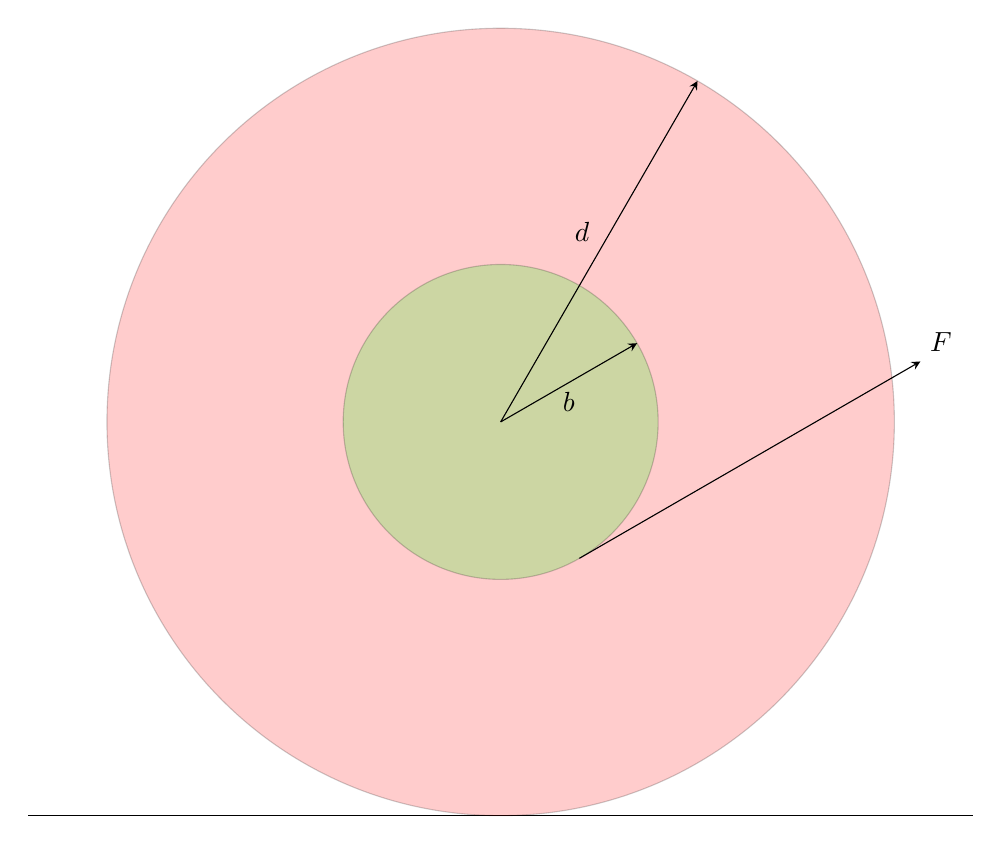
\begin{tikzpicture}
		\def\d{5};
		\def\b{2};
		\def\angle{30};
		
		\draw ({-(\d+1)},-\d) -- ({\d+1},-\d);
		
		\filldraw [fill = red, opacity = 0.2] (0,0) circle [radius = \d];
		
		\filldraw [fill = green, opacity = 0.2] (0,0) circle [radius = \b];

		\draw [-stealth] (0,0) -- (\angle:\b) node [midway, below] {$b$};
		\draw [-stealth] (0,0) -- (2*\angle:\d) node [midway, above left] {$d$};
		
		\draw [-stealth] ({-(90-\angle)}:\b) -- ++(\angle:5) node [above right] {$F$};
	\end{tikzpicture}
\end{example}

\begin{solution}
	For the torque about the IAOR to be zero, $F$ must be in the direction of the tangent from the point of contact to the inner cylinder.\\
	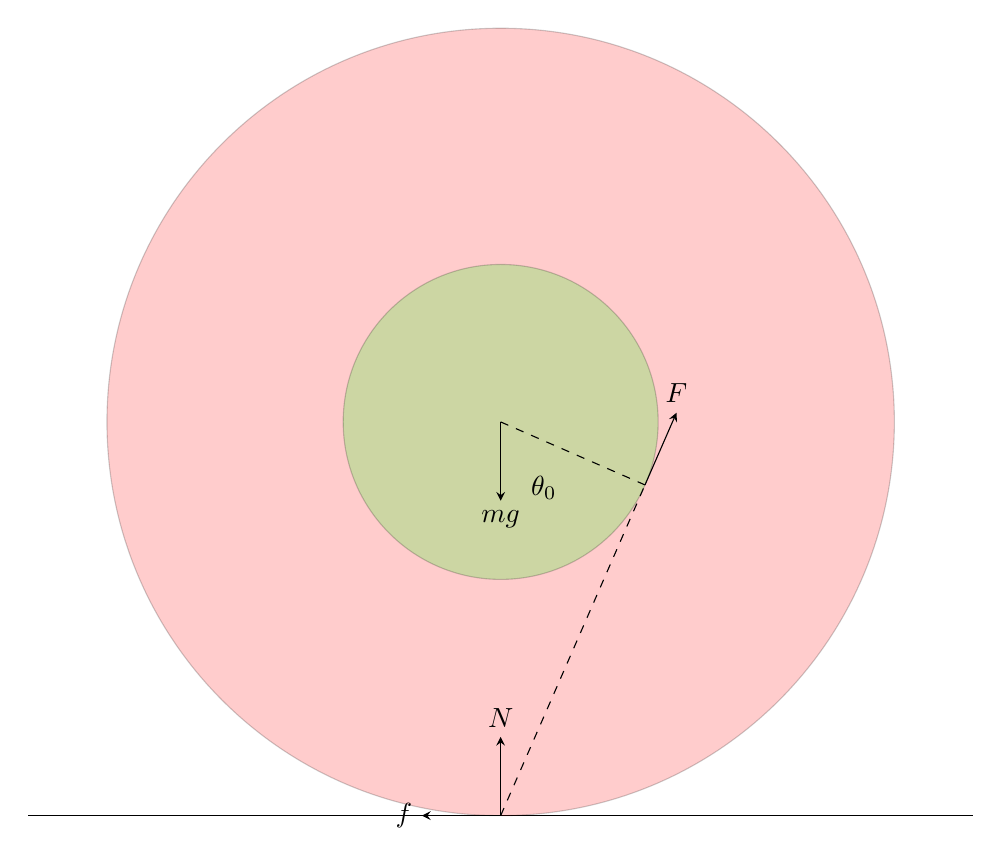
\begin{tikzpicture}
		\def\d{5};
		\def\b{2};
		\def\angle{66.42};
		
		\coordinate (point of application of force) at ($ (0,\d) + ({-90 + \angle}:\b) $);
		
		\draw ({-(\d+1)},0) -- ({\d+1},0);
		
		\filldraw [fill = red, opacity = 0.2] (0,\d) circle [radius = \d];
		
		\filldraw [fill = green, opacity = 0.2] (0,\d) circle [radius = \b];
		
		\draw [dashed] (0,\d) -- ++({-90 + \angle}:\b);
		
		\draw [dashed] (0,0) -- (point of application of force);
		
		\node at ($ (0,\d) + ({-90 + (\angle/2)}:1) $) {$\theta_0$};
		
		%forces
		\draw [-stealth] (0,0) -- ++(90:1) node [above] {$N$};
		\draw [-stealth] (0,0) -- ++(180:1) node [left] {$f$};
		\draw [-stealth] (0,\d) -- ++(-90:1) node [below] {$mg$};
		\draw [-stealth] (point of application of force) -- ++(\angle:1) node [above] {$F$};
	\end{tikzpicture}\\
	As the body is stationary, 
	\begin{align*}
		F \sin \theta_0 + N &= mg\\
		F \cos \theta_0 &= f
	\end{align*}
	About the centre, as $\tau = 0$,
	\begin{align*}
		\cos \theta_0 &= \dfrac{b}{d}		
	\end{align*}
	Therefore,
	\begin{align*}
		Fb &= fd
	\end{align*}
	If $\theta < \theta_0$,
	\begin{align*}
		F \cos \theta - f &= m a_{\text{COM}}\\
		F \sin \theta + N &= mg\\
		f d - b F &= k m d^2 \alpha\\
		&= k m d a_{\text{COM}}
	\end{align*}
	Solving,
	\begin{align*}
		a_{\text{COM}} &= \dfrac{F d (\cos \theta - \sfrac{b}{d})}{m d (1 + k)}
	\end{align*}
\end{solution}

\begin{example}
	A disk is of mass $m_1$ is fixed at its centre and is rotating with $\omega_0$. A system with a small brake pad is arranged such that the brake pad touches the disk, as shown. Find the angular velocity of the disk as a function of time.\\
	\begin{tikzpicture}
		\coordinate (pivot) at (0,0);
		
		\def\R{2};
		\def\r{2};
		\def\l{10};
		\def\y{5};
		\def\F{1};
		\def\angle{30};
		
		\coordinate (disk centre) at (\l/3, -\R);
		\coordinate (disk top) at ($ (disk centre) + (90:\R) $);
		\coordinate (disk left) at ($ (disk centre) + (180:\R) $);
		\coordinate (disk right) at ($ (disk centre) + (0:\R) $);
		\coordinate (disk contact) at ($ (disk centre) + (90:\R) $);
		
		\coordinate (pulley centre) at (\l, -\y);
		\coordinate (pulley top) at ($ (pulley centre) + (90:\r) $);
		\coordinate (pulley left) at ($ (pulley centre) + (180:\r) $);
		\coordinate (pulley right) at ($ (pulley centre) + (0:\r) $);
		\coordinate (pulley connector) at ($ (pulley centre) + (90:\y) $);
		
		\coordinate (m3) at ($ (pulley left) + (-90:5) $);
		
		\coordinate (m4) at ($ (pulley right) + (-90:5) $);
		
		\draw (pivot) -- (disk top) -- (pulley connector) -- (pulley centre);
		
		\fill (pivot) circle [radius = 2pt] node [below] {pivot};
		
		\draw (disk centre) circle [radius = \R] node [below] {$m_1$};
		
		\fill (disk centre) circle [radius = 1pt];
		
		\draw (disk centre) -- ++(\angle:\R) node [midway, fill = white] {$R$};
		
		\draw (pulley centre) circle [radius = \r] node [below] {$m_2$};
		
		\fill (pulley centre) circle [radius = 1pt];
		
		\draw (pulley centre) -- ++(\angle:\r) node [midway, fill = white] {$r$};
		
		\draw (pulley left) -- (m3);
		\fill (m3) circle [radius = 2 pt] node [left] {$m_3$};
		
		\draw (pulley right) -- (m4);
		\fill (m4) circle [radius = 2 pt] node [right] {$m_4$};
		
		\draw [-stealth, green] (pulley centre) -- ++(90:\F) node [right] {$\tilde{T}$};
		\draw [-stealth, green] (pulley left) -- ++(-90:\F) node [left] {$T_2$};
		\draw [-stealth, green] (pulley right) -- ++(-90:\F) node [right] {$T_1$};
		
		\draw [-stealth, blue] (m3) -- ++(90:\F) node [left] {$T_2$};
		\draw [-stealth, blue] (m3) -- ++(-90:\F) node [left] {$m_3 g$};
		\draw [-stealth, blue] ($ (m3) + (180:1) $) -- ++(90:\F/2) node [left] {$a$};
		
		\draw [-stealth, red] (m4) -- ++(90:\F) node [left] {$T_1$};
		\draw [-stealth, red] (m4) -- ++(-90:\F) node [left] {$m_3 g$};
		\draw [-stealth, red] ($ (m4) + (0:1) $) -- ++(-90:\F/2) node [left] {$a$};
		
		\draw [-stealth, orange] (pulley connector) -- ++(-90:\F) node [right] {$\tilde{T}$};
		\draw [-stealth, orange] (disk contact) -- ++(90:\F) node [left] {$N$};
		
		\draw [-stealth, purple] (disk contact) -- ++(-90:\F) node [left] {$N$};
		\draw [-stealth, purple] (disk contact) -- ++(180:\F) node [above] {$\mu N$};
	\end{tikzpicture}
\end{example}

\begin{solution}
	For the pulley and the masses,
	\begin{align*}
		m_4 g - T_1 &= m_4 a\\
		T_2 - m_3 g &= m_3 a\\
		T_1 r - T_2 r &= \dfrac{1}{2} m_2 r^2 \alpha\\
		\tilde{T} &= T_1 + T_2 + m_2 g
	\end{align*}
	For the lever, as $\tau = 0$ about the pivot point,
	\begin{align*}
		0 &= -\tilde{T} L + N \dfrac{L}{3}\\
		\therefore N &= 3 \tilde{T}
	\end{align*}
	For the disk,
	\begin{align*}
		f R &= \dfrac{1}{2} m_1 R^2 \alpha\\
		\therefore \alpha &= \dfrac{3 \mu \tilde{T}}{\sfrac{1}{2} \cdot m_1 R}
	\end{align*}
	Therefore,
	\begin{align*}
		\omega &= \omega_0 - \dfrac{6 \mu \tilde{T}}{m_1 R} \cdot t
	\end{align*}
\end{solution}

\begin{example}
	A sphere of radius $b$ is fixed to the ground. A sphere of radius $a$ is placed on its top. The smaller sphere is rolling without slipping.\\
	\begin{tikzpicture}
		\coordinate (pivot) at (0,0);
		
		\def\a{2};
		\def\b{5};
		\def\angle{30};		
		\def\F{1};
		
		\coordinate (fixed sphere centre) at (90:\b);
		\coordinate (moving sphere centre) at (90:{2*\b + \a});
		\coordinate (moving sphere centre at angle) at ($ (fixed sphere centre) + (\angle:{\b + \a}) $);
		
		\draw (fixed sphere centre) circle [radius = \b];
		\draw (moving sphere centre) circle [radius = \a];
		
		\draw [dashed] ($ (fixed sphere centre) + (\angle:{\b + \a}) $) circle [radius = \a];
		
		%dimensions
		\draw [dashed] (fixed sphere centre) -- ++(90:\b) node [midway, fill = white] {$b$};
		
		\draw [dashed] (moving sphere centre) -- ++(90:\a) node [midway, fill = white] {$a$};
		
		\draw [dashed] (fixed sphere centre) -- ++(\angle:{\b + \a});
		\draw [dashed] (fixed sphere centre) -- ++(0:\b);
			\node at ($ (fixed sphere centre) + ({\angle/2}:1)$) {$\theta$};
		
		%forces
		\draw [-stealth] (moving sphere centre at angle) -- ++({180 + \angle}:\F) node [below left] {$m g \sin \theta$};
		\draw [-stealth] (moving sphere centre at angle) -- ++({-(90 - \angle)}:\F) node [below right] {$m g \sin \theta$};
		
		\draw [-stealth] (moving sphere centre at angle) -- ++(\angle:\F) node [above right] {$N$};
	\end{tikzpicture}
\end{example}

\begin{solution}
	\begin{align*}
		m g \sin \theta - N &= m \dfrac{v_{\text{COM}}^2}{a + b}
	\end{align*}
	When the ball loses contact, $N = 0$. Therefore,
	\begin{align*}
		m g \sin \theta &= m \dfrac{v_{\text{COM}}^2}{a + b}
	\end{align*}
	By COME,
	\begin{align*}
		0 &= - m g (a + b) (1 - \sin \theta) + \dfrac{1}{2} \left( \dfrac{2}{5} m a^2 \right) \omega^2 + \dfrac{1}{2} m v_{\text{COM}}^2
	\end{align*}
	As the ball is purely rolling,
	\begin{align*}
		v_{\text{COM}} &= \omega a
	\end{align*}
	Solving,
	\begin{align*}
		\theta &= \sin^{-1} \left( \dfrac{10}{17} \right)
	\end{align*}
\end{solution}

\begin{example}
	A pool ball of radius $R$ is at rest on the ground. A cue hits the ball at $h$ from the ground. Find $h$ such that the ball starts purely rolling.
\end{example}

\begin{solution}
	By COLM,
	\begin{align*}
		p_0 &= m v_{\text{COM}}
	\end{align*}
	By COAM, with respect to the IAOR,
	\begin{align*}
		h p_0 &= \dfrac{7}{5} m R^2 \omega
	\end{align*}
	As the ball is purely rolling,
	\begin{align*}
		v_{\text{COM}} &= \omega R
	\end{align*}
	Therefore,
	\begin{align*}
		h m v_{\text{COM}} &= \dfrac{7}{5} m R^2 \omega\\
		\therefore h m \omega R &= \dfrac{7}{5} m R^2 \omega\\
		\therefore h &= \dfrac{7}{5} R
	\end{align*}
\end{solution}

\begin{example}
	A pool ball of mass $m$ and radius $R$ is at rest on a rough ground. The coefficient of friction between the ball and the ground is $\mu$. A cue hits the ball at $R$ from the ground. Find 
\end{example}

\begin{solution}
	\begin{align*}
		p_0 &= m v_{\text{COM}}
	\end{align*}
	\begin{align*}
		m a_{\text{COM}} &= -\mu m g\\
		\therefore v_{\text{COM}} &= -\mu g t
	\end{align*}
	\begin{align*}
		\mu m g R &= \dfrac{2}{5} m R^2 \alpha\\
		\therefore \alpha &= \dfrac{5 \mu g}{2 R}\\
		\therefore \omega &= \dfrac{5 \mu g}{2 R} t
	\end{align*}
	The ball will start at some $t_1$, such that
	\begin{align*}
		v_{\text{COM}}(t_1) &= \omega(t_1) R\\
		\dfrac{p_0}{m} - \mu g t_1 &= \dfrac{5 \mu g }{2 R} t_1 R\\
		\therefore t &= \dfrac{2 p_0}{7 m}
	\end{align*}
\end{solution}

\end{document}